\documentclass[11pt]{exam}

% \usetikzlibrary{calc,patterns}

\newcommand{\Version}{1} 
\newcommand{\Solutions}{0} 

% TEST SPECIFIC INFORMATION
\ifnum \Version=1 \newcommand{\TestName}{MATH 2552 In-Class Worksheet: Final Exam Review} \fi


% LOAD PACKAGES
\usepackage{amsmath} % allows for align env and other things
\usepackage{amssymb} % 
\usepackage{mathtools} % allows for single apostrophe
\usepackage{enumitem} % allows for alpha lettering in enumerated lists
\usepackage{lastpage}
\usepackage{array} % for table alignments

\usepackage{graphicx} % if images are needed
\usepackage{wrapfig} % to allow text wrapping

\addpoints

\usepackage{pgfplots} % for surfaces (chapter 7)
\usepackage{tikz-3dplot} 
\pgfplotsset{compat=1.9}
\usetikzlibrary{decorations.pathmorphing,patterns} % for some tikz diagrams
% ~~~~~~~~~~~~~~~~~~~~~~~~~~~~~~~~~~~~
% INITIALS
\newcommand{\Initials}{\textit{\Course, \TestName. Your initials: \underline{\hspace{3cm}}} \vspace{1pt}}

\newcommand{\InitialsLeft}{\noindent \hspace{-18pt}\textit{\Course, \TestName. Your initials: \underline{\hspace{3cm}}} \vspace{1pt}}

\newcommand{\InitialsRight}{\begin{flushright}\textit{\Course, \TestName. Your initials: \underline{\hspace{3cm}}} \vspace{1pt}\end{flushright}}

% ADJUST FIRST LINE IN PARAGRAPH INDENTATION 
\setlength\parindent{0pt}

% FONT FORMAT
\renewcommand*\rmdefault{lmss} % change font to lat mod ss

% ADJUST MARGINS 
\usepackage[a4paper, tmargin=0.8in,bmargin=0.8in,left=1in,right=1in]{geometry}

% TIKZ DIAGRAMS
\usepackage{color}
\usepackage{tikz}  \usetikzlibrary{arrows} 
\usetikzlibrary{calc} 

% COURSE SPECIFIC INFORMATION
\newcommand{\Course}{Math 2552, Differential Equations}
\newcommand{\Instructors}{}

\newcommand{\LastPage}{\begin{center}\textit{This page may be used for scratch work. Please indicate clearly if you would like your work on this page to be graded. }\end{center}   }

% DERIVATIVES
\newcommand{\dfdy}{{\frac{df}{dy}}} % 
\newcommand{\dydt}{{\frac{dy}{dt}}} % 
\newcommand{\dxdt}{{\frac{dx}{dt}}} % 
\newcommand{\dydx}{{\frac{dy}{dx}}} % 
\newcommand{\dydtt}{{\frac{d ^2y}{dt^2}}} % 
\newcommand{\dydxx}{{\frac{d^2y}{dx^2}}} % 
\newcommand{\dydttt}{{\frac{d^3y}{dt^3}}} % 

\newcommand{\ddt}{{\frac{d}{dt}}} % 
\newcommand{\ddx}{{\frac{d}{dx}}} % 
\newcommand{\ddy}{{\frac{d}{dy}}} % 
\newcommand{\dudt}{{\frac{du}{dt}}} % 
\newcommand{\dvdx}{{\frac{dv}{dx}}} % 
\newcommand{\dxdtt}{{\frac{d^2x}{dt^2}}} % 
\newcommand{\dzdt}{{\frac{dz}{dt}}} % 

% COLORS FOR SOLUTIONS
\definecolor{DarkBlue}{rgb}{0.0,0.2,0.4} % 
\definecolor{DarkRed}{rgb}{0.4,0.1,0.1} % 
\definecolor{DarkGreen}{rgb}{0.0,0.25,0.15} % 

% ADJUST FIRST LINE IN PARAGRAPH INDENTATION 
\setlength\parindent{0pt}

% FONT FORMAT
\renewcommand*\rmdefault{lmss} % change font to lat mod ss


% HEADERS AND FOOTERS
\pagestyle{headandfoot}
\runningfooter{}{}{}
\runningheader{}{}{\textit{\TestName, Page \thepage \ of \pageref{LastPage}} }
% \headheight 42pt % distance from top of page to top of header
% \headsep 24pt % space between header and top of body


\begin{document}
    
\vspace*{-1cm}

\begin{center}
{\Large \TestName}
\end{center}
% \newcommand{\ID}{Please print your first name: \framebox{\strut\hspace{4.2cm}}, last name: \framebox{\strut\hspace{4.2cm}}, \\[2pt] and the remaining digits of your GTID:  \framebox{\strut $9$}\framebox{\strut $0$}\framebox{\strut\hspace{0.19cm}}\framebox{\strut\hspace{0.19cm}}\framebox{\strut\hspace{0.19cm}}\framebox{\strut\hspace{0.19cm}}\framebox{\strut\hspace{0.19cm}}\framebox{\strut\hspace{0.19cm}}\framebox{\strut\hspace{0.19cm}}.}

% \ID

\vspace{6pt}
\textbf{Instructions}: this worksheet is not being collected but students are encouraged to work on the following questions on their own and/or with other students to prepare for the final exam. You don't need to turn this one in! 
\def\dm{\displaystyle}

% \begin{center}

    \textbf{Complex Solutions to First Order Systems}
    \begin{align*}
        \lambda_k &= \alpha + i \beta, \ \beta \ne 0 , \ \vec v_k = \vec a + i \vec b, \quad 
        \vec x_k = e^{\alpha t} (\vec a \cos \beta t - \vec b \sin \beta t), 
        \quad 
        \vec x_{k+1} = e^{\alpha t} (\vec a \sin \beta t + \vec b \cos \beta t)
    \end{align*}

    \vspace{4pt}
    \textbf{Second Order Homogeneous Constant Coefficient}
    \begin{tabular}{ p{4.2cm} p{4.6cm} }
        
        $\lambda_1, \lambda_2$ &  general solution 
        \\[2pt] \hline 
        real distinct &  $c_1 e^{\lambda_1 t} + c_2 e^{\lambda_2 t}$\\       
        real repeated, $\lambda_1 = \lambda_2$ & $c_1 e^{\lambda_1 t} + c_2 t e^{\lambda_1 t}$\\
        complex, $\lambda_1 = \alpha + i \beta$ & $e^{\alpha t} \left( c_1 \cos \beta t + c_2 \sin \beta t \right)$\\[2pt] \hline
    \end{tabular}    
    
    \vspace{4pt}
    \textbf{Second Order Homogeneous Cauchy-Euler}
    \begin{tabular}{ p{6.2cm} p{6cm} }
        roots &  general solution 
        \\[2pt] \hline 
        real distinct, $m_1 \ne m_2$ &  $c_1 t^{m_1} + c_2 t^{m_2}$\\       
        real repeated, $m = m_1 = m_2$ & $c_1 t^{m} + c_2 t^m \ln(t)$\\
        complex, $m_1 = \alpha + i \beta$ & $c_1t^{\alpha}\cos(\beta \ln(t)) + c_2t^{\alpha}\sin(\beta \ln (t))$\\[2pt] \hline
    \end{tabular}
    
    \vspace{4pt}
    \textbf{Undetermined Coefficients} 
    \begin{align*}
        P_n &= a_0t^n + a_1t^{n-1} \ldots + a_n, \
        Q_n = A_0t^n + A_1t^{n-1} \ldots + A_n, \       
        R_n = B_0t^n + B_1t^{n-1} \ldots + B_n     
    \end{align*}
    \vspace{-0.4cm}
    \setlength{\extrarowheight}{0.05cm}
    \begin{tabular}{ p{3.9cm} p{5cm} }
        $g(t)$ &  particular solution $y_p(t)$ 
        \\[2pt] \hline $P_n(t)$  & $t^s Q_n$   \\        
        $P_n(t)e^{\alpha t}$ &  $t^s e^{\alpha t}Q_n$\\       
        $P_n(t)e^{\alpha t}\sin(\beta t)$ & $t^s e^{\alpha t} \left(\cos(\beta t)Q_n+\sin(\beta t) R_n\right)$\\
        $P_n(t)e^{\alpha t}\cos(\beta t)$ & $t^s e^{\alpha t} \left(\cos(\beta t)Q_n+\sin(\beta t) R_n\right)$\\[2pt] \hline
    \end{tabular}
    \setlength{\extrarowheight}{0.0cm}

    \vspace{14pt}
    \textbf{Variation of Parameters}    
    \begin{align*}
        \text{scalar form: } y_p &= v_1 (t) y_1(t) + v_2(t) y_2(t) , \quad 
        v_1 = - \int \frac{y_2(t)g(t)}{W[y_1,y_2]}dt , \quad 
        v_2 = \int \frac{y_1(t)g(t)}{W[y_1,y_2]} dt \\
        \text{first-order system: }\vec x \, ' &= P \vec x + \vec g(t), \quad \vec x_p = X(t) \int X^{-1}(t) \vec g(t) \, dt
    \end{align*}        
    
    \vspace{1pt}
    \textbf{Matrix Inverse}  
    $$\text{if } A= \begin{pmatrix} a& b\\c&d\end{pmatrix}, \ \text{then } A^{-1} = \frac{1}{|A|}\begin{pmatrix} d&-b\\-c&a\end{pmatrix}$$
\end{center}
% \def\dm{\displaystyle}

\begin{center}
    {\bf Elementary Laplace Transforms}\\[2pt]
\end{center}
$
\hspace*{-.5em}
\begin{array}{lllllll}
 1.  & 1 \quad  & 1/s,\quad s>0 & \qquad  \ \quad & 10.  & t^n e^{at}\  \quad  & \frac{n!}{(s-a)^{n+1}},\quad s>a\\[1ex] 
 2.  & e^{at} \quad  & 1/(s-a),\quad s>a  & \qquad  \ \quad & 11. & u_c(t)\ \ (c\ge 0) \quad  & e^{-cs}/s,\quad s>0 \\[1ex]
 3.  & t^n  \quad  & n!/s^{n+1},\quad s>0 & \qquad  \ \quad & 12.  & u_c(t)f(t-c)\  \quad  & \dm e^{-cs} F(s), \ c\ge 0 \\[1ex] 
 4.  & \sin(at) \quad  & a/(s^2+a^2),\quad s>0  & \qquad  \ \quad & 13.  & e^{ct}f(t) \quad  & \dm F(s-c) \\[1ex] 
 5.  & \cos(at) \quad  & s/(s^2+a^2),\quad s>0  & \qquad  \ \quad & 14.  & t^n f(t) \quad  & \dm (-1)^n F^{(n)}(s) \\[1ex]
 6.  & e^{at}\sin(bt) \quad  & \dm\frac{b}{(s-a)^2+b^2},\quad s>a  & \qquad  \ \quad & 15. & f(t-T) = f(t) \quad  & \dm \frac{1}{1-e^{-sT}}\int_0^Te^{-st}f(t)\,dt \\[1ex]
 7.  & e^{at}\cos(bt) \quad  & \dm\frac{s-a}{(s-a)^2+b^2},\quad s>a & \qquad  \ \quad &  16. & \delta(t-c) & e^{-cs}\\[1ex]
 8.  & f'(t) \  \quad  &  sF(s) - f(0) & \qquad  \ \quad & 17. & f\ast g & F(s)G(s) \\[1ex]
 9.  & f''(t) \  \quad   & s^2F(s) - sf(0) - f'(0) & \qquad  \ \quad &  & & \\[1ex]
\end{array} 
$

\subsection*{Exercises}

    \begin{questions}

        \question Compute the Laplace Transform of the periodic function shown below. The function satisfies $y(t+2a) = y(t)$ for all $t\ge 0$. 
        \begin{center}
        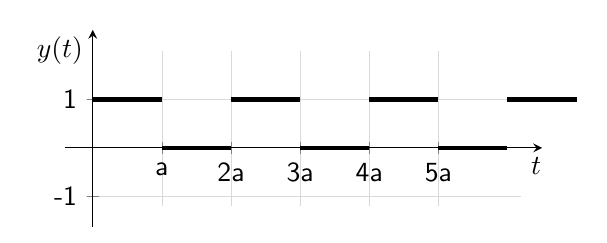
\begin{tikzpicture}[scale=1] 
            \begin{axis}[
            width=2.8in,
            height=1.4in,
            clip=false,
            axis lines=middle,
            xmin=-.1,xmax=6.2,
            ymin=-1.2, ymax=2,
            xtick={1,2,3,4,5},
            xticklabels={a,2a,3a,4a,5a},
            ytick={-1,0,1},
            yticklabels={-1,0,1},        
            axis line style={shorten >=-7.5pt, shorten <=-7.5pt},
            xlabel=$t$,
            ylabel=$y(t)$,
            xlabel style={at={(ticklabel* cs:1)},anchor=north west},
            ylabel style={at={(ticklabel* cs:1)},anchor= east},
            grid style={line width=.2pt, draw=gray!30},
            grid=both,
            ]
            \addplot[black,samples=50,domain=0:1,ultra thick] {1};% 
            \addplot[black,samples=50,domain=1:2,ultra thick] {0};% 
            \addplot[black,samples=50,domain=2:3,ultra thick] {1};% 
            \addplot[black,samples=50,domain=3:4,ultra thick] {0};% 
            \addplot[black,samples=50,domain=4:5,ultra thick] {1};% 
            \addplot[black,samples=50,domain=5:6,ultra thick] {0};% 
            \addplot[black,samples=50,domain=6:7,ultra thick] {1};% 
            \end{axis}
        \end{tikzpicture}             
        \end{center}
        

        \vfill    
    
        \question Solve the following IVP: $y'' + 2y' + 2y = \delta(t - \pi),  \quad y(0) = y'(0) = 1$. 

        \vfill

        \newpage
    
        \question A system obeys the equation $\displaystyle \dydt = f(y) = y^2 -4y - 5 = (y+1)(y-5)$, for $y \in \mathbb R$, and $t \ge 0$. The equilibrium points are located at $y = -1$ and $y=5$. For $y \in \mathbb R$ determine whether $y$ is concave up or concave down. Sketch a few integral curves of the DE. 

        \vfill 


        \question Use the convolution theorem to solve the IVP below. You may leave your answer in terms of a convolution integral. Assume $g(t)$ is an unknown function whose Laplace Transform is $G(s)$. 
        $$4y''+4y'+17y = g(t), \quad y(0) = y'(0) = 0$$

        \vfill

        \newpage

        \question In the following dynamical systems a coefficient matrix and its eigenvalues are given. Sketch the phase portrait. 
        \begin{enumerate}
            \item[a)] $\vec x \, ' = A\vec x$, where $A=\begin{pmatrix} 1&-4\\1&-3\end{pmatrix}$, and $\lambda_1=\lambda_2 = -1$.
            \vfill
            \item[b)] $\vec x \, ' = A\vec x$, where $A=\begin{pmatrix} 3&-2\\4&-1\end{pmatrix}$, and $\lambda_1=1+2i, \lambda_2 =1-2i $. 
            \vfill
        \end{enumerate}


    \question % \textit{4.5 \#24, \#25 verbatim} \\
    Determine a suitable form for the particular solution $y_p(t)$ if the method of undetermined coefficients is to be used. The homogeneous solution is given. 
    
    \begin{enumerate}
        \item[a)] $y''+y = t(1+\sin t)$, $y_h = c_1\cos t + c_2 \sin t$. 
        \item[b)] $y'' - 5y' + 6y = e^t \cos(2t) + e^{2t} (3t + 4) \sin(2t)$, $y_h = c_1e^{2t} + c_2 e^{3t}$. 
    \end{enumerate}
    \vfill
    \newpage 

    \question Consider the first order, constant coefficient, linear initial value problem $\vec x \, ' = A\vec x, \ \vec x (0) = \vec x_0$, where $\vec x \, ' = A\vec x$ and $\vec x = \vec x(t)$. The vector $\vec x_0$, and the eigenvalues and eigenvectors of $A$ are as follows. 
$$\lambda_1 = -4, \  v_1 = \begin{pmatrix}1\\0\\0 \end{pmatrix} , \quad \lambda_2 = -2+3i, \  v_2 = \begin{pmatrix} 0\\1\\i \end{pmatrix}, \quad \lambda_3 = \bar{\lambda_2}, \ v_3 = \bar{v_2}, \quad \vec x_0 = \begin{pmatrix} 3\\0\\4\end{pmatrix}$$
\begin{parts}
    \part Write down the general solution to the system of differential equations $\vec x \, ' = A \vec x$ in terms of real-valued functions. 
    \vspace{4cm}
    \part Solve the initial value problem. Please state the solution to the initial value problem clearly and please show your work. 
\end{parts}

\newpage

\question Solve the following Cauchy-Euler equation: $t^2y'' - 3ty' + 3y = 0, \quad t > 0$. 

\vfill

\question Given that $y_1 = e^t$ is a solution of $y''-y=0$, use the reduction of order method to determine a second solution to this DE. 
\vfill 

    \end{questions}

    
\end{document}